\section{Ergebnisse}

\subsection{Experimentdesign}
Das experimentelle Design wurde in sechs diskrete Phasen (EXP-001 bis EXP-006) sowie nachgeschaltete Optimierungsphasen und Architektur-Experimente unterteilt, um Systemgenauigkeit und Ressourceneffizienz systematisch zu evaluieren. Die Experimente gliedern sich in Stage~A (Klassifikation) und Stage~B (Detektion), wobei Stage~B eine Migration der Basisarchitektur von YOLOv8-Nano zu YOLO11n umfasst.

\subsection{Klassifikationsphase (EXP-001 bis EXP-004)}
Die erste Phase verglich drei Architekturen auf demselben Validierungssplit: ein Scratch-CNN (EXP-001, Val.~Accuracy~\SI{61.00}{\percent}), MobileNetV2 mit gefrorenem Backbone (EXP-002, \SI{84.28}{\percent}) und MobileNetV2 mit Fine-Tuning (EXP-003, \SI{87.42}{\percent}). Ziel war zu prüfen, wie stark Transfer Learning den Sprung von einem kleinen, direkt trainierten Netz zu einem robusteren Modell verbessert \cite{yosinski2014transferable}.

EXP-001 zeigte starkes Overfitting mit verrauschten Validierungskurven und systematischen Fehlklassifikationen (Papier und Metall wurden häufig als Plastik fehlinterpretiert). EXP-002 profitierte deutlich vom Transfer Learning (\SI{84.28}{\percent} Genauigkeit), erreichte aber noch kein zufriedenstellendes Niveau. EXP-003 lieferte mit \SI{87.42}{\percent} Genauigkeit das stabilste Modell und reduzierte die Fehlklassifikationen erheblich -- insbesondere für Glass (F1: 0,94). Der vollständige Vergleich aller vier Klassifikationsmodelle ist in Abbildung~\ref{fig:stagea-acc} dargestellt.

\subsection{Quantisierung (EXP-004)}
Das beste Keras-Modell (EXP-003) wurde per TensorFlow Lite exportiert. Dabei wurden ein FP32-Modell (volle 32-Bit-Gleitkommapräzision) und anschließend ein voll quantisiertes INT8-Modell erzeugt. Für die Kalibrierung kam eine repräsentative Stichprobe von 100 Bildern zum Einsatz \cite{deng2020model}. Die Klassifikationsleistung blieb dabei nahezu identisch (\SI{87.35}{\percent} vs.\ \SI{87.42}{\percent} des FP32-Modells), während die Modellgröße um den Faktor 9 auf \SI{2.61}{\mega\byte} sank.

\subsection{Detektionsphase YOLOv8 (EXP-005 bis EXP-009)}
Die zweite Projektphase drehte sich um Objekterkennung. Zunächst wurde ein YOLOv8-Nano-Modell auf einem einfachen Benchmark trainiert (EXP-005). Dieses Modell erreichte zwar eine scheinbar hohe Validierungsgenauigkeit von \SI{82.3}{\percent} mAP50 (mean Average Precision bei IoU-Schwelle 0,5). Diese hohe Metrik erwies sich jedoch bei einer detaillierten Fehleranalyse als Artefakt eines extremen Hintergrund-Overfittings (Background Leakage): Da der Canny-Edge-Auto-Labeler die kontrastreichen Kanten und Helligkeitsgradienten des Schreibtischrahmens umschloss, lernte das Netzwerk nicht die Müllobjektspezifika selbst, sondern korrelierte die Geometrie der gesamten Arbeitsfläche mit der Zielklasse. Dies erklärt die hohe Genauigkeit auf dem monotonen Test-Set der Tischoberfläche, führte aber zu einem vollständigen Versagen (mAP50 nahe \SI{0}{\percent}) bei Tests auf abweichenden Hintergründen. Dieser GIGO-Effekt (Abschnitt~\ref{sec:method-gigo}) zwang zur Verfeinerung der Datengrundlage. Spätere Modelle (EXP-006, EXP-009) trainierten auf gemischten Wild-Datensätzen und dem bereinigten TrashNet-Datensatz \cite{yang2016classification}.

\subsection{Architekturmigration: YOLO11n (EXP-013 bis EXP-016)}
\label{sec:exp-yolo11}
Im dritten Abschnitt der Detektionsphase wurde die Basisarchitektur von YOLOv8-Nano (\SI{3.01}{Mio.}\ Parameter) auf YOLO11n (\SI{2.58}{Mio.}\ Parameter) migriert \cite{ultralyticsyolov8}. YOLO11n ist kompakter (6,3 GFLOPs) und erreicht auf dem fusionierten mira\_v2-Datensatz (\num{4024} Bilder, TACO + TrashNet) einen ausgeglichenen mAP50 von \SI{55.1}{\percent} (EXP-013). Ein systematischer Vergleich evaluierte anschließend den Einfluss zusätzlicher Datenquellen:

\begin{itemize}
    \item \textbf{EXP-013 (Baseline):} TACO~\cite{proenca2020taco} + TrashNet~\cite{yang2016classification} (\num{4024}~Bilder) $\rightarrow$ mAP50~\SI{55.1}{\percent}
    \item \textbf{EXP-014 (+Roboflow):} Zusätzlich Roboflow Trash Detection \cite{roboflow2023trash} $\rightarrow$ mAP50~\SI{60.7}{\percent} \textbf{(Bestes Modell)}
    \item \textbf{EXP-015 (+WaRP):} Roboflow ersetzt durch WaRP~Waste~Detection \cite{warp2024dataset} $\rightarrow$ mAP50~\SI{56.0}{\percent}
    \item \textbf{EXP-016 (WaRP-only):} Ausschließlich WaRP $\rightarrow$ mAP50~\SI{58.8}{\percent} (jedoch ohne \textit{trash}-Klasse)
\end{itemize}

EXP-014 erzielt den besten Gesamtmittelwert (+5,6~pp über EXP-013), mit dem stärksten Zuwachs bei Trash (+11,3~pp); Glass sinkt leicht (-6,3~pp, von \SI{56.5}{\percent} auf \SI{50.2}{\percent}). Der WaRP-Datensatz (EXP-015) verbessert Glass signifikant (+24,8~pp), senkt aber Trash drastisch (-12,6~pp), da WaRP keine Trash-Klasse enthält. Der vollständige Modellvergleich ist in Abbildung~\ref{fig:heatmap-4datasets} als Heatmap dargestellt. Die Trainingsmetriken des besten Modells (EXP-014) zeigt Abbildung~\ref{fig:yolo11n}.

\subsection{Modellvergleich der Klassifikation (Stage A)}
\begin{figure}[H]
    \centering
    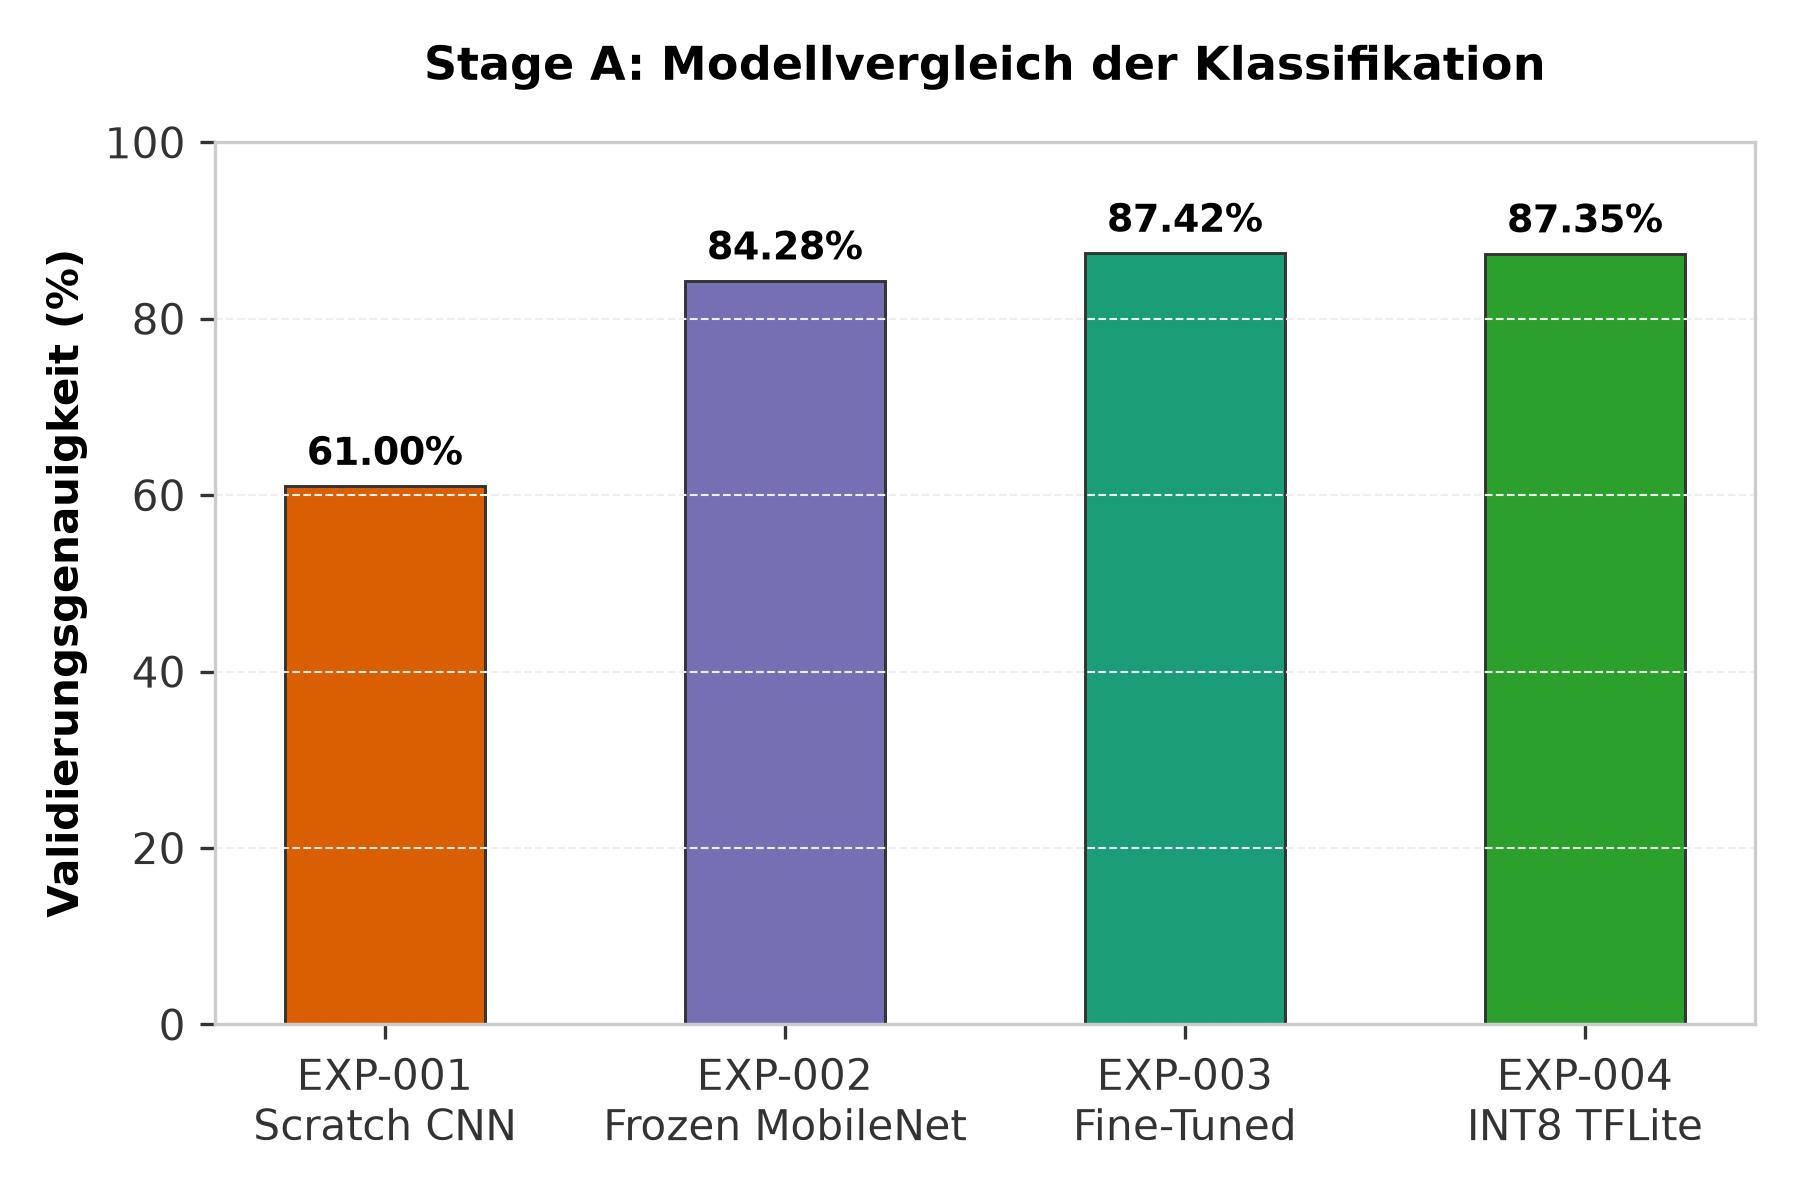
\includegraphics[width=0.75\textwidth, keepaspectratio]{figures/stagea-acc-comparison.png}
    \caption{Vergleich der Validierungsgenauigkeit der vier Klassifikationsmodelle (Stage A).}
    \label{fig:stagea-acc}
\end{figure}

\subsection{Detaillierter Klassifikationsvergleich}
Tabelle~\ref{tab:class-results} zeigt die vollständigen Metriken inklusive Loss, Latenz und Dateigröße. Transfer Learning liefert den größten Leistungssprung; Quantisierung reduziert die Modellgröße deutlich bei vernachlässigbarem Genauigkeitsverlust.

\begin{table}[h]
    \centering
    \caption{Vergleich der Klassifikationsmodelle}
    \label{tab:class-results}
    \begin{tabular}{lcccc}
        \toprule
        \textbf{Modell} & \textbf{Val. Acc.} & \textbf{Val. Loss} & \textbf{Latenz} & \textbf{Größe} \\
        \midrule
        EXP-001 Baseline CNN & \SI{61.00}{\percent} & 1,0633 & \SI{5.81}{\milli\second} & \SI{15.22}{\mega\byte} \\
        EXP-002 Frozen MobileNetV2 & \SI{84.28}{\percent} & 0,5659 & \SI{38.00}{\milli\second} & \SI{8.49}{\mega\byte} \\
        EXP-003 Fine-Tuned MobileNetV2 & \SI{87.42}{\percent} & 0,3148 & \SI{40.00}{\milli\second} & \SI{23.48}{\mega\byte} \\
        EXP-004 INT8 TFLite & \SI{87.35}{\percent} & -- & \SI{10.32}{\milli\second} & \SI{2.61}{\mega\byte} \\
        \bottomrule
    \end{tabular}
\end{table}

\subsection{Detektionsmetriken (Stage B)}
Die vollständigen Metriken inklusive GPU/CPU-Latenz sind in Tabelle~\ref{tab:yolo-results} dokumentiert.

\begin{table}[h]
    \centering
    \caption{Detektionsresultate: Architektur- und Datensatzvergleich (EXP-013 bis EXP-016)}
    \label{tab:yolo-results}
    \small
    \begin{tabular}{llcccc}
        \toprule
        \textbf{Experiment} & \textbf{Datensatz} & \textbf{mAP50} & \textbf{mAP50-95} & \textbf{GPU} & \textbf{CPU} \\
        \midrule
        EXP-013 YOLO11n & TACO+TrashNet & \SI{55.10}{\percent} & \SI{49.80}{\percent} & \SI{3.60}{\milli\second} & \SI{45.20}{\milli\second} \\
        EXP-014 YOLO11n & +Roboflow & \textbf{\SI{60.70}{\percent}} & \SI{50.60}{\percent} & \SI{1.80}{\milli\second} & \SI{46.00}{\milli\second} \\
        EXP-015 YOLO11n & +WaRP & \SI{56.00}{\percent} & \SI{45.10}{\percent} & \SI{1.50}{\milli\second} & \SI{45.50}{\milli\second} \\
        EXP-016 YOLO11n & WaRP-only & \SI{58.80}{\percent} & \SI{43.20}{\percent} & \SI{1.20}{\milli\second} & \SI{44.80}{\milli\second} \\
        \bottomrule
    \end{tabular}
\end{table}

\begin{figure}[H]
    \centering
    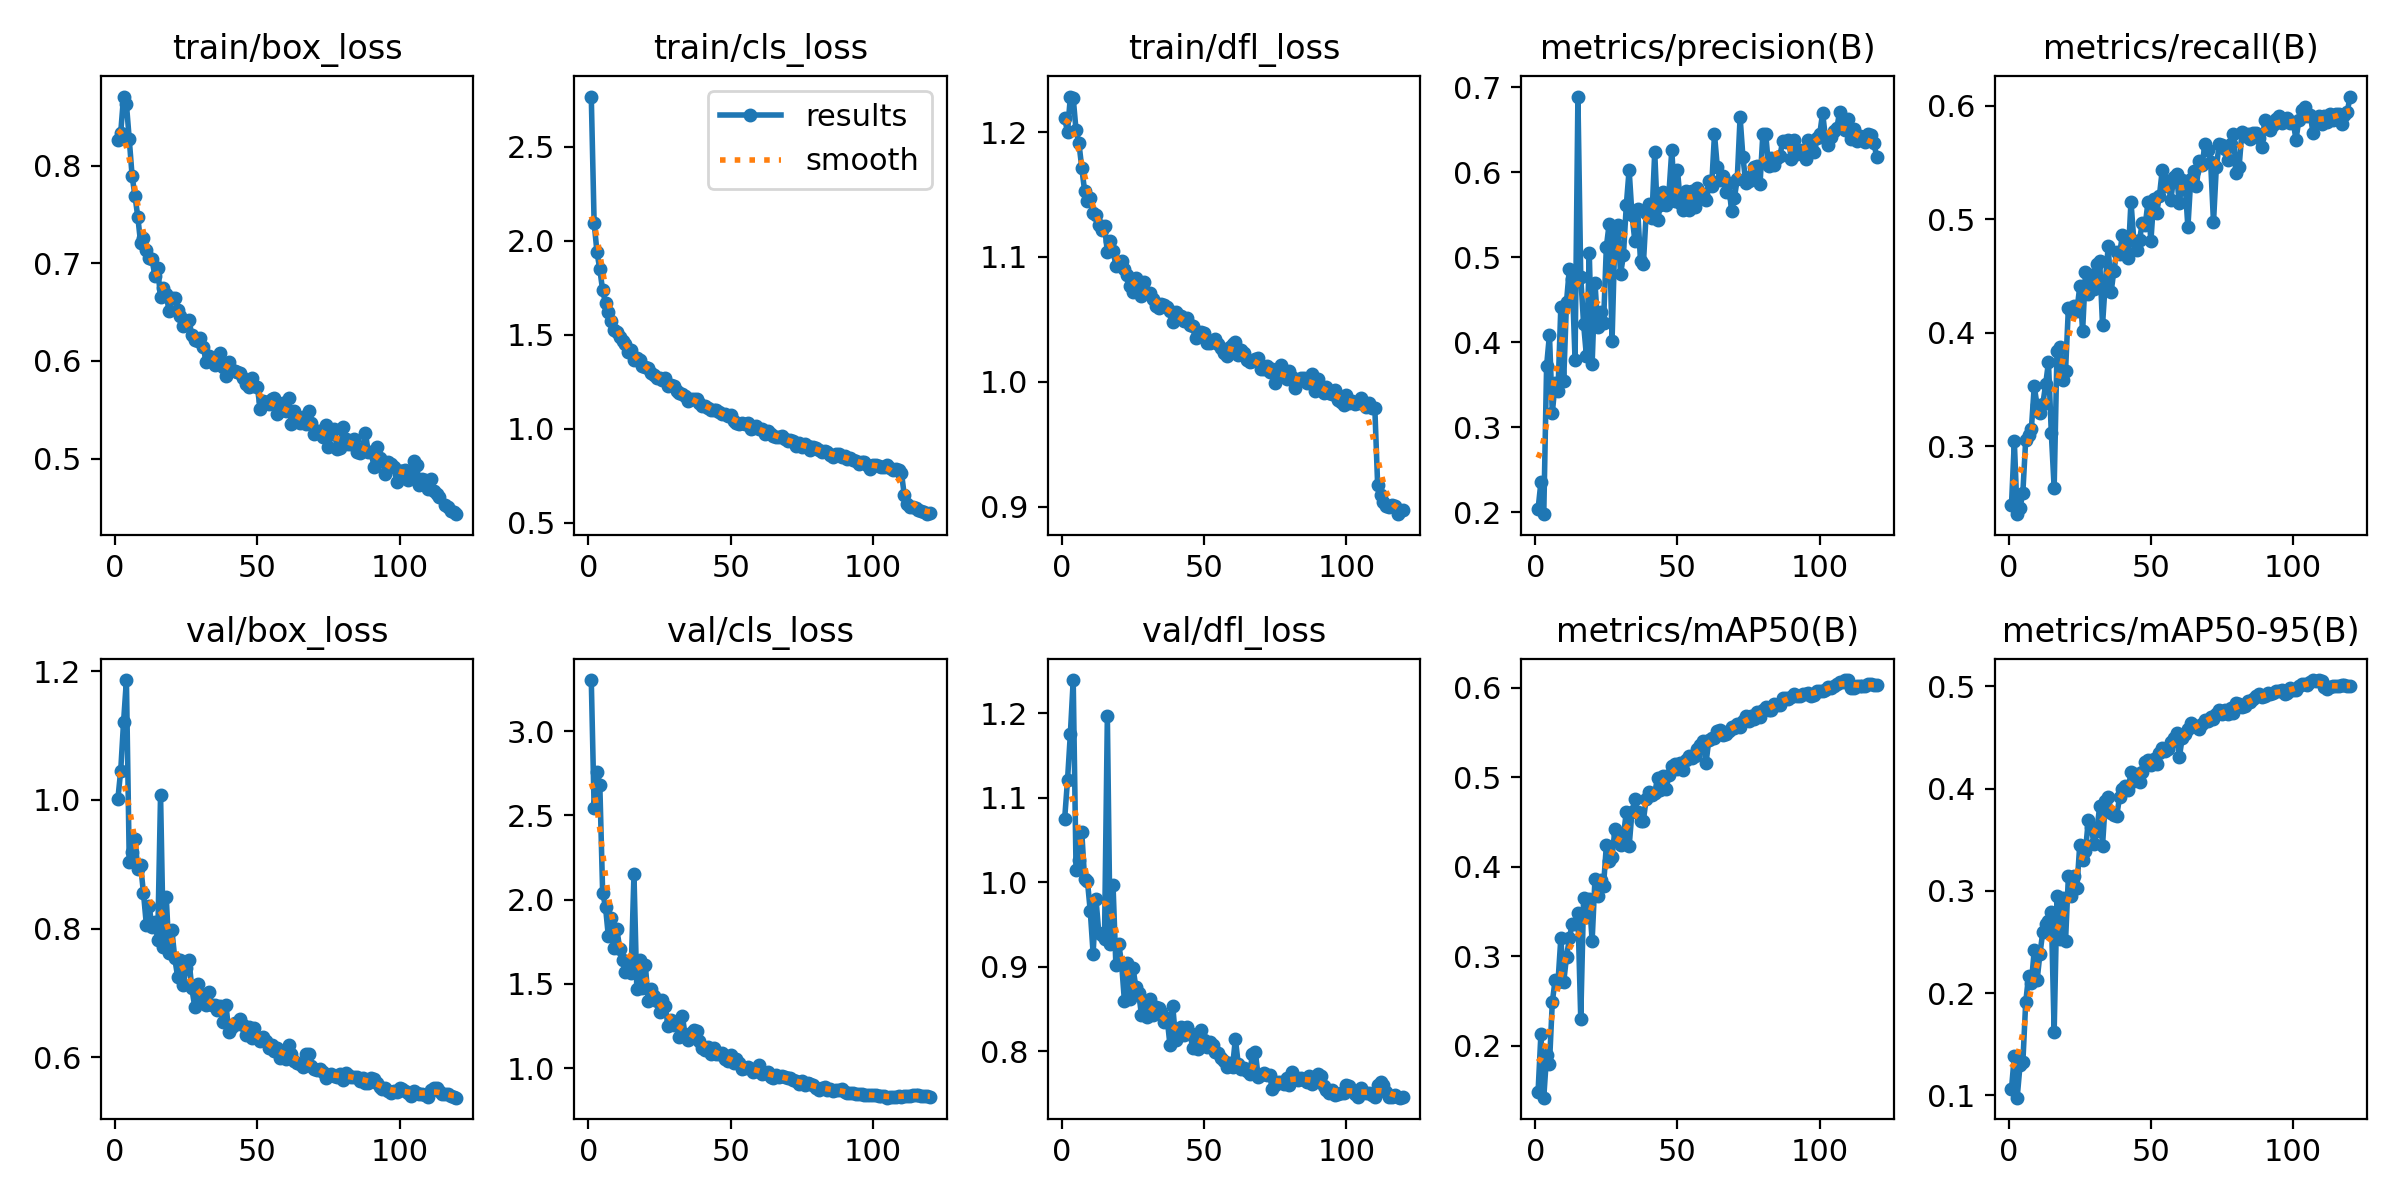
\includegraphics[width=0.75\textwidth, keepaspectratio]{figures/exp14-results.png}
    \caption{Trainingsmetriken des besten YOLO11n-Detektors (EXP-014). Durch die Datenfusion aus TACO, TrashNet und Roboflow wird ein robuster mAP50 von \SI{60.7}{\percent} erreicht.}
    \label{fig:yolo11n}
\end{figure}

\subsection{Architekturvergleich und Fehlermatrix-Heatmap}
Abbildung~\ref{fig:heatmap-4datasets} vergleicht die klassenspezifische mAP50 der vier YOLO11n-Modelle als Heatmap. Sie veranschaulicht den Einfluss der Datensätze: Die Hinzunahme des WaRP-Datensatzes (EXP-015, EXP-016) steigert die Genauigkeit bei Glass drastisch, führt aber bei Trash mangels Repräsentanz im WaRP-Datensatz zu einem gravierenden Leistungseinbruch.

\begin{figure}[H]
    \centering
    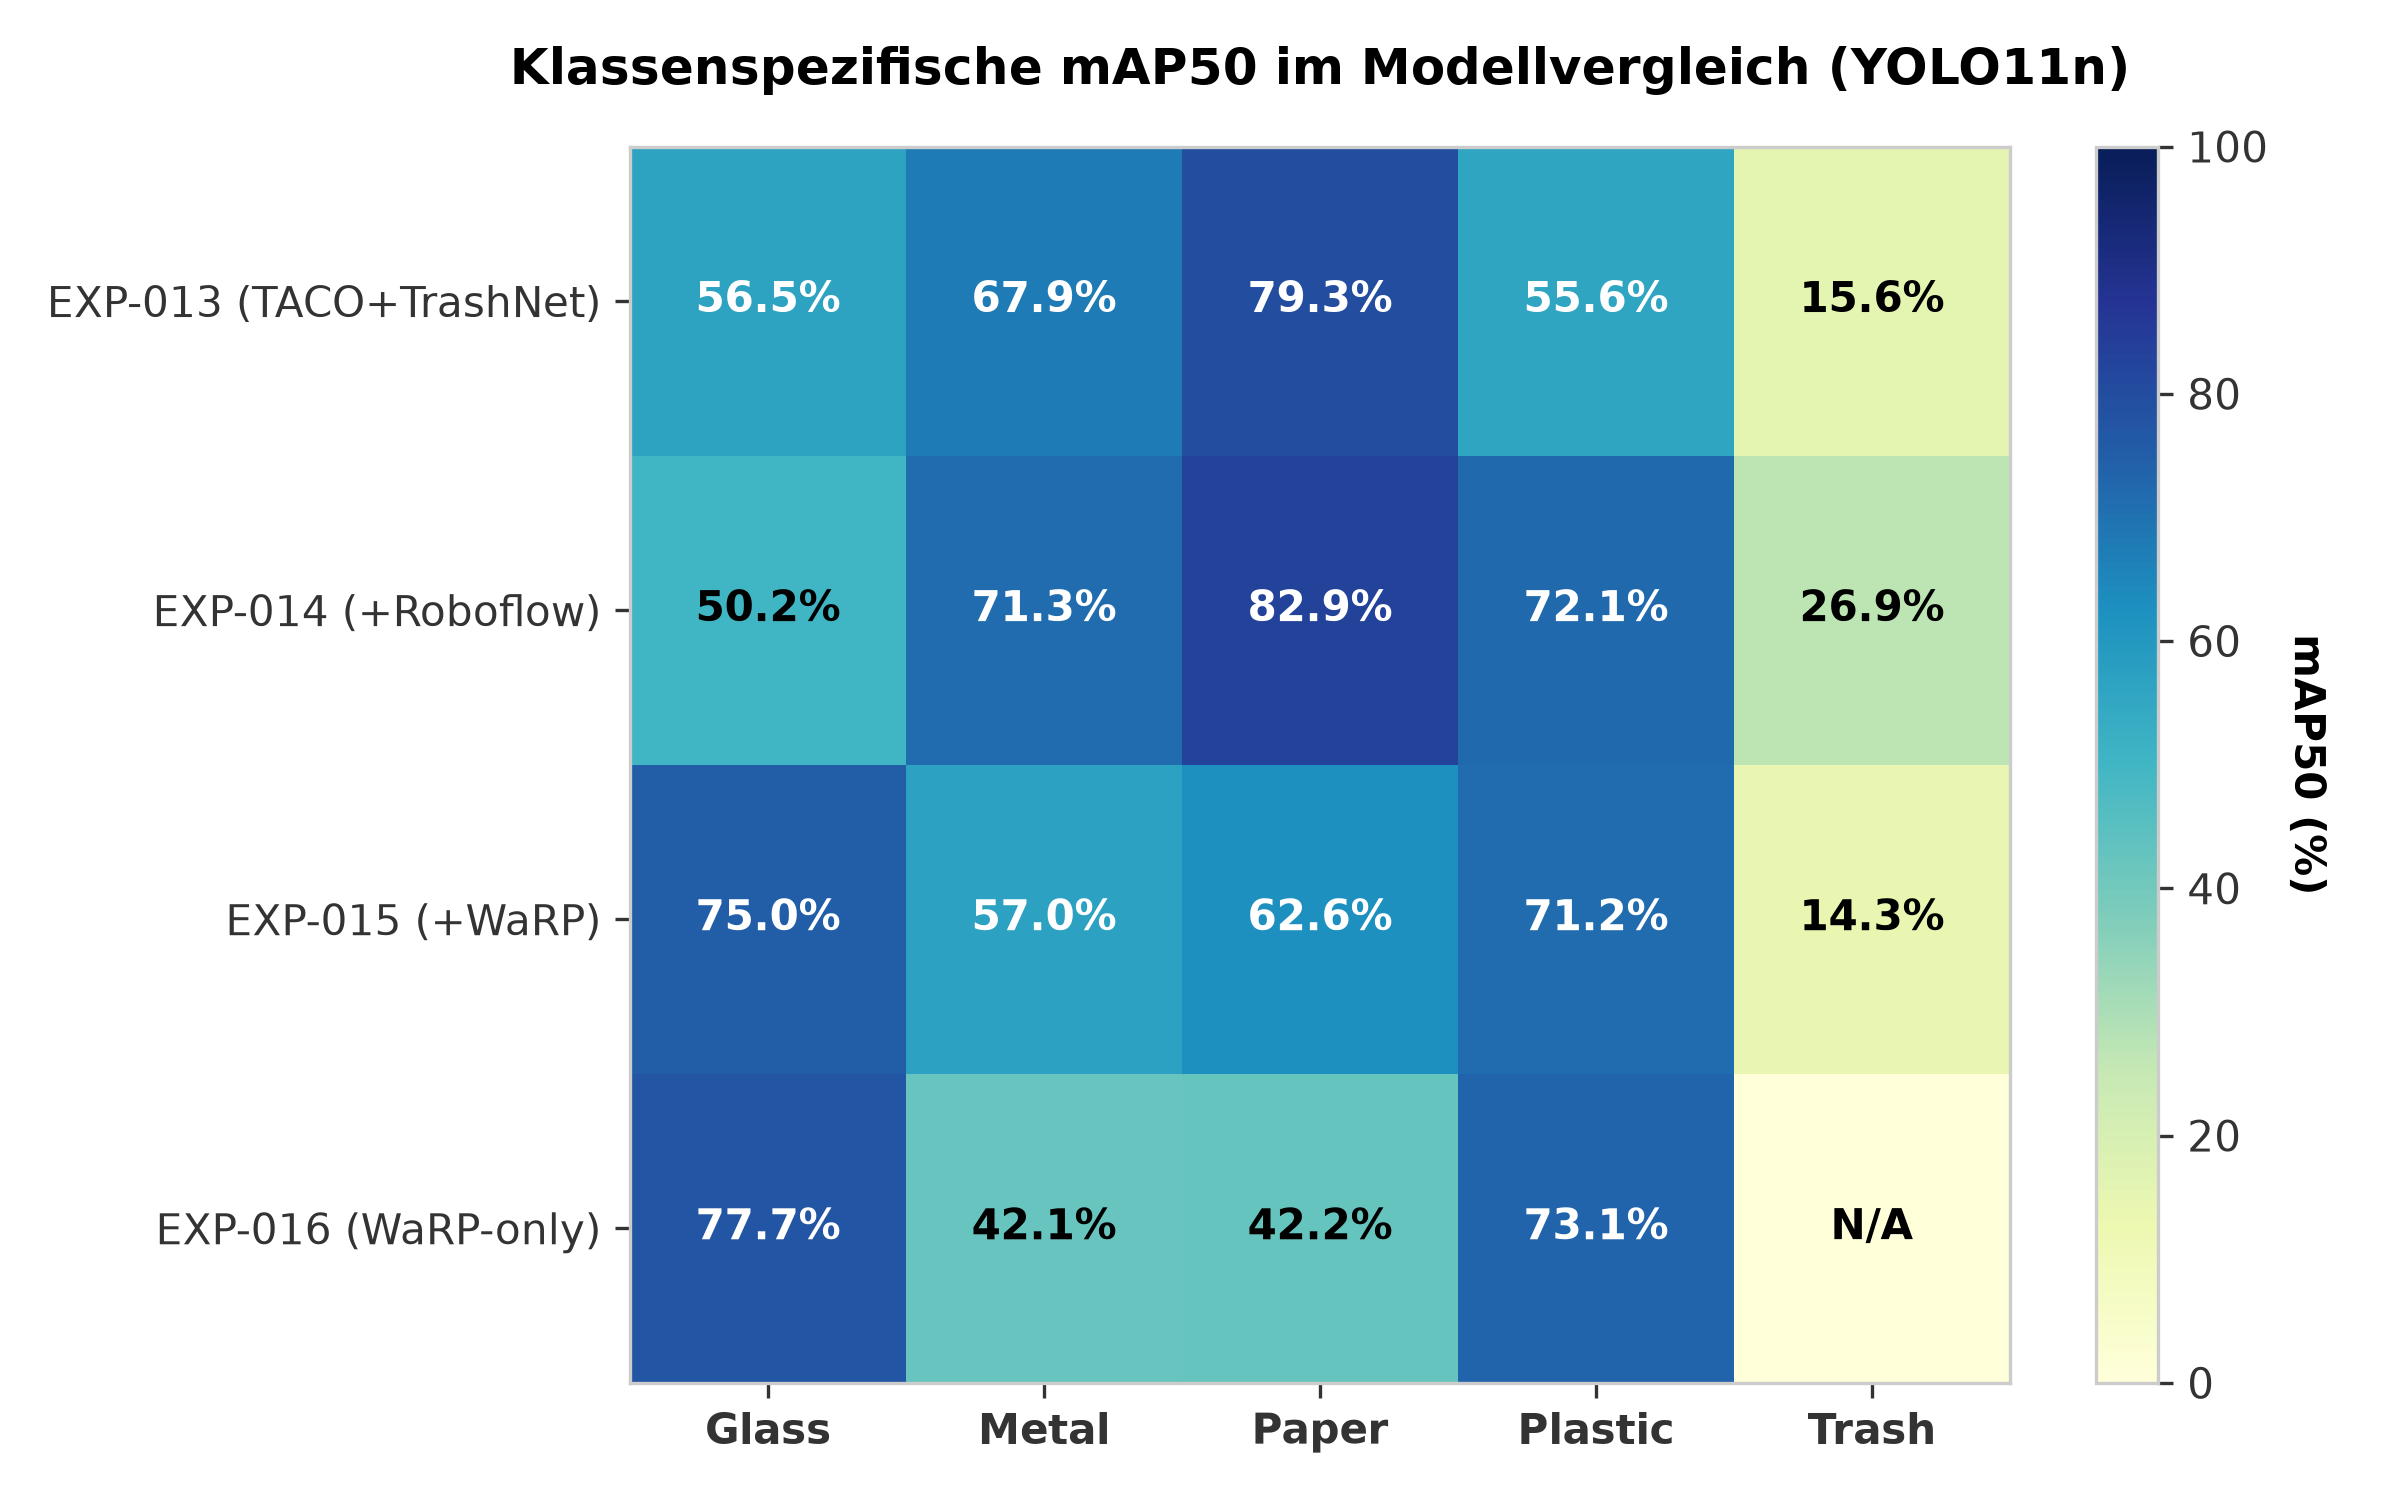
\includegraphics[width=0.8\textwidth, keepaspectratio]{figures/heatmap-4datasets.png}
    \caption{Heatmap-Modellvergleich der klassenspezifischen mAP50-Ergebnisse (YOLO11n-Experimente EXP-013 bis EXP-016).}
    \label{fig:heatmap-4datasets}
\end{figure}

\subsection{Per-Class-Analyse: Bestes Detektionsmodell (EXP-014)}
Tabelle~\ref{tab:exp014-class} zeigt die klassenspezifischen Validierungsergebnisse. Paper bleibt die stärkste Klasse, Trash die schwächste.

\begin{table}[h]
    \centering
    \caption{Klassenspezifische Metriken von EXP-014 (YOLO11n, TACO+TrashNet+Roboflow)}
    \label{tab:exp014-class}
    \small
    \begin{tabular}{lccccc}
        \toprule
        \textbf{Klasse} & \textbf{Precision} & \textbf{Recall} & \textbf{mAP50} & \textbf{mAP50-95} & \textbf{Instanzen} \\
        \midrule
        Glass   & \num{0.580} & \num{0.521} & \num{0.502} & \num{0.400} & \num{336} \\
        Metal   & \num{0.670} & \num{0.699} & \num{0.713} & \num{0.613} & \num{439} \\
        Paper   & \num{0.820} & \num{0.772} & \textbf{\num{0.829}} & \num{0.745} & \num{474} \\
        Plastic & \num{0.715} & \num{0.699} & \num{0.721} & \num{0.601} & \num{1316} \\
        Trash   & \num{0.523} & \num{0.230} & \num{0.269} & \num{0.173} & \num{561} \\
        \bottomrule
    \end{tabular}
\end{table}

Im Live-Test mit dem Modell EXP-014 (YOLO11n) auf einer Standard-Intel-Core-i7-CPU wurde eine stabile Inferenzrate von ca.\ 21,7\,FPS (Frames per Second, Latenz ca.\ \SI{46.0}{\milli\second}) gemessen, was für einen kontinuierlichen Sortierprozess ausreicht. Alle Latenzen der GPU-Spalte in Tabelle \ref{tab:yolo-results} wurden auf einer Nvidia T4 Cloud-GPU erfasst, um eine Vergleichbarkeit mit Standard-Benchmarks zu gewährleisten. Auf der geplanten Zielhardware (Raspberry Pi Zero 2W bzw.\ Raspberry Pi 4) wird nach vorläufigen Compiler-Simulationen durch den LiteRT-INT8-Export eine Latenz von ca.\ \SI{90}{\milli\second} bis \SI{120}{\milli\second} (ca.\ \num{8} bis \num{11} FPS) erwartet. Dies macht die Kopplung mit einem schnellen Tracker wie ByteTrack~\cite{zhang2022bytetrack} zur Bewegungsprädiktion zwingend erforderlich.

\subsection{Praxistest (Field Benchmark)}
Um die Generalisierungsfähigkeit der Modelle zu prüfen, wurde ein Field-Benchmark auf dem mira\_v2-Validierungsset (\num{805}~Bilder, fünf Klassen, Konfidenzschwelle~\num{0.5}) durchgeführt. Tabelle~\ref{tab:field-bench} und Abbildung~\ref{fig:field-benchmark-f1} vergleichen die Praxisergebnisse aller Modelle. Das Modell \texttt{mira\_exp011\_int8.tflite} erzielte dabei \SI{0}{\percent} Precision und Recall: INT8-Quantisierung verschiebt die Konfidenzscores nach unten, sodass bei der Standardschwelle~\num{0.5} keine Detektionen übrig bleiben; bei einer niedrigeren Schwelle (ca.~\num{0.25}) arbeitet das Modell wieder normal.

\begin{table}[h]
    \centering
    \caption{Modellvergleich im realen Praxistest (Field Benchmark)}
    \label{tab:field-bench}
    \small
    \begin{tabular}{lcccccc}
        \toprule
        \textbf{Modell} & \textbf{TP} & \textbf{FP} & \textbf{FN} & \textbf{Precision} & \textbf{Recall} & \textbf{F1} \\
        \midrule
        \textbf{mira\_exp014.pt} & \textbf{669} & \textbf{51} & \textbf{170} & \textbf{\SI{92.9}{\percent}} & \textbf{\SI{79.7}{\percent}} & \textbf{\SI{85.8}{\percent}} \\
        mira\_exp014\_int8.tflite & 492 & 20 & 347 & \SI{96.1}{\percent} & \SI{58.6}{\percent} & \SI{72.8}{\percent} \\
        mira\_exp015.pt & 572 & 68 & 267 & \SI{89.4}{\percent} & \SI{68.2}{\percent} & \SI{77.3}{\percent} \\
        mira\_exp015\_int8.tflite & 579 & 67 & 260 & \SI{89.6}{\percent} & \SI{69.0}{\percent} & \SI{78.0}{\percent} \\
        mira\_exp013.pt & 589 & 82 & 250 & \SI{87.8}{\percent} & \SI{70.2}{\percent} & \SI{78.0}{\percent} \\
        mira\_exp013\_int8.tflite & 475 & 30 & 364 & \SI{94.1}{\percent} & \SI{56.6}{\percent} & \SI{70.7}{\percent} \\
        mira\_exp011.pt & 624 & 94 & 215 & \SI{86.9}{\percent} & \SI{74.4}{\percent} & \SI{80.2}{\percent} \\
        mira\_exp009\_int8.tflite & 624 & 107 & 215 & \SI{85.4}{\percent} & \SI{74.4}{\percent} & \SI{79.5}{\percent} \\
        mira\_exp006.pt & 696 & 139 & 259 & \SI{83.4}{\percent} & \SI{72.9}{\percent} & \SI{77.8}{\percent} \\
        mira\_exp006\_int8.tflite & 375 & 197 & 473 & \SI{65.6}{\percent} & \SI{44.2}{\percent} & \SI{52.8}{\percent} \\
        mira\_exp011\_int8.tflite & 0 & 0 & 839 & \SI{0.0}{\percent} & \SI{0.0}{\percent} & \SI{0.0}{\percent} \\
        \bottomrule
    \end{tabular}
\end{table}

\begin{figure}[H]
    \centering
    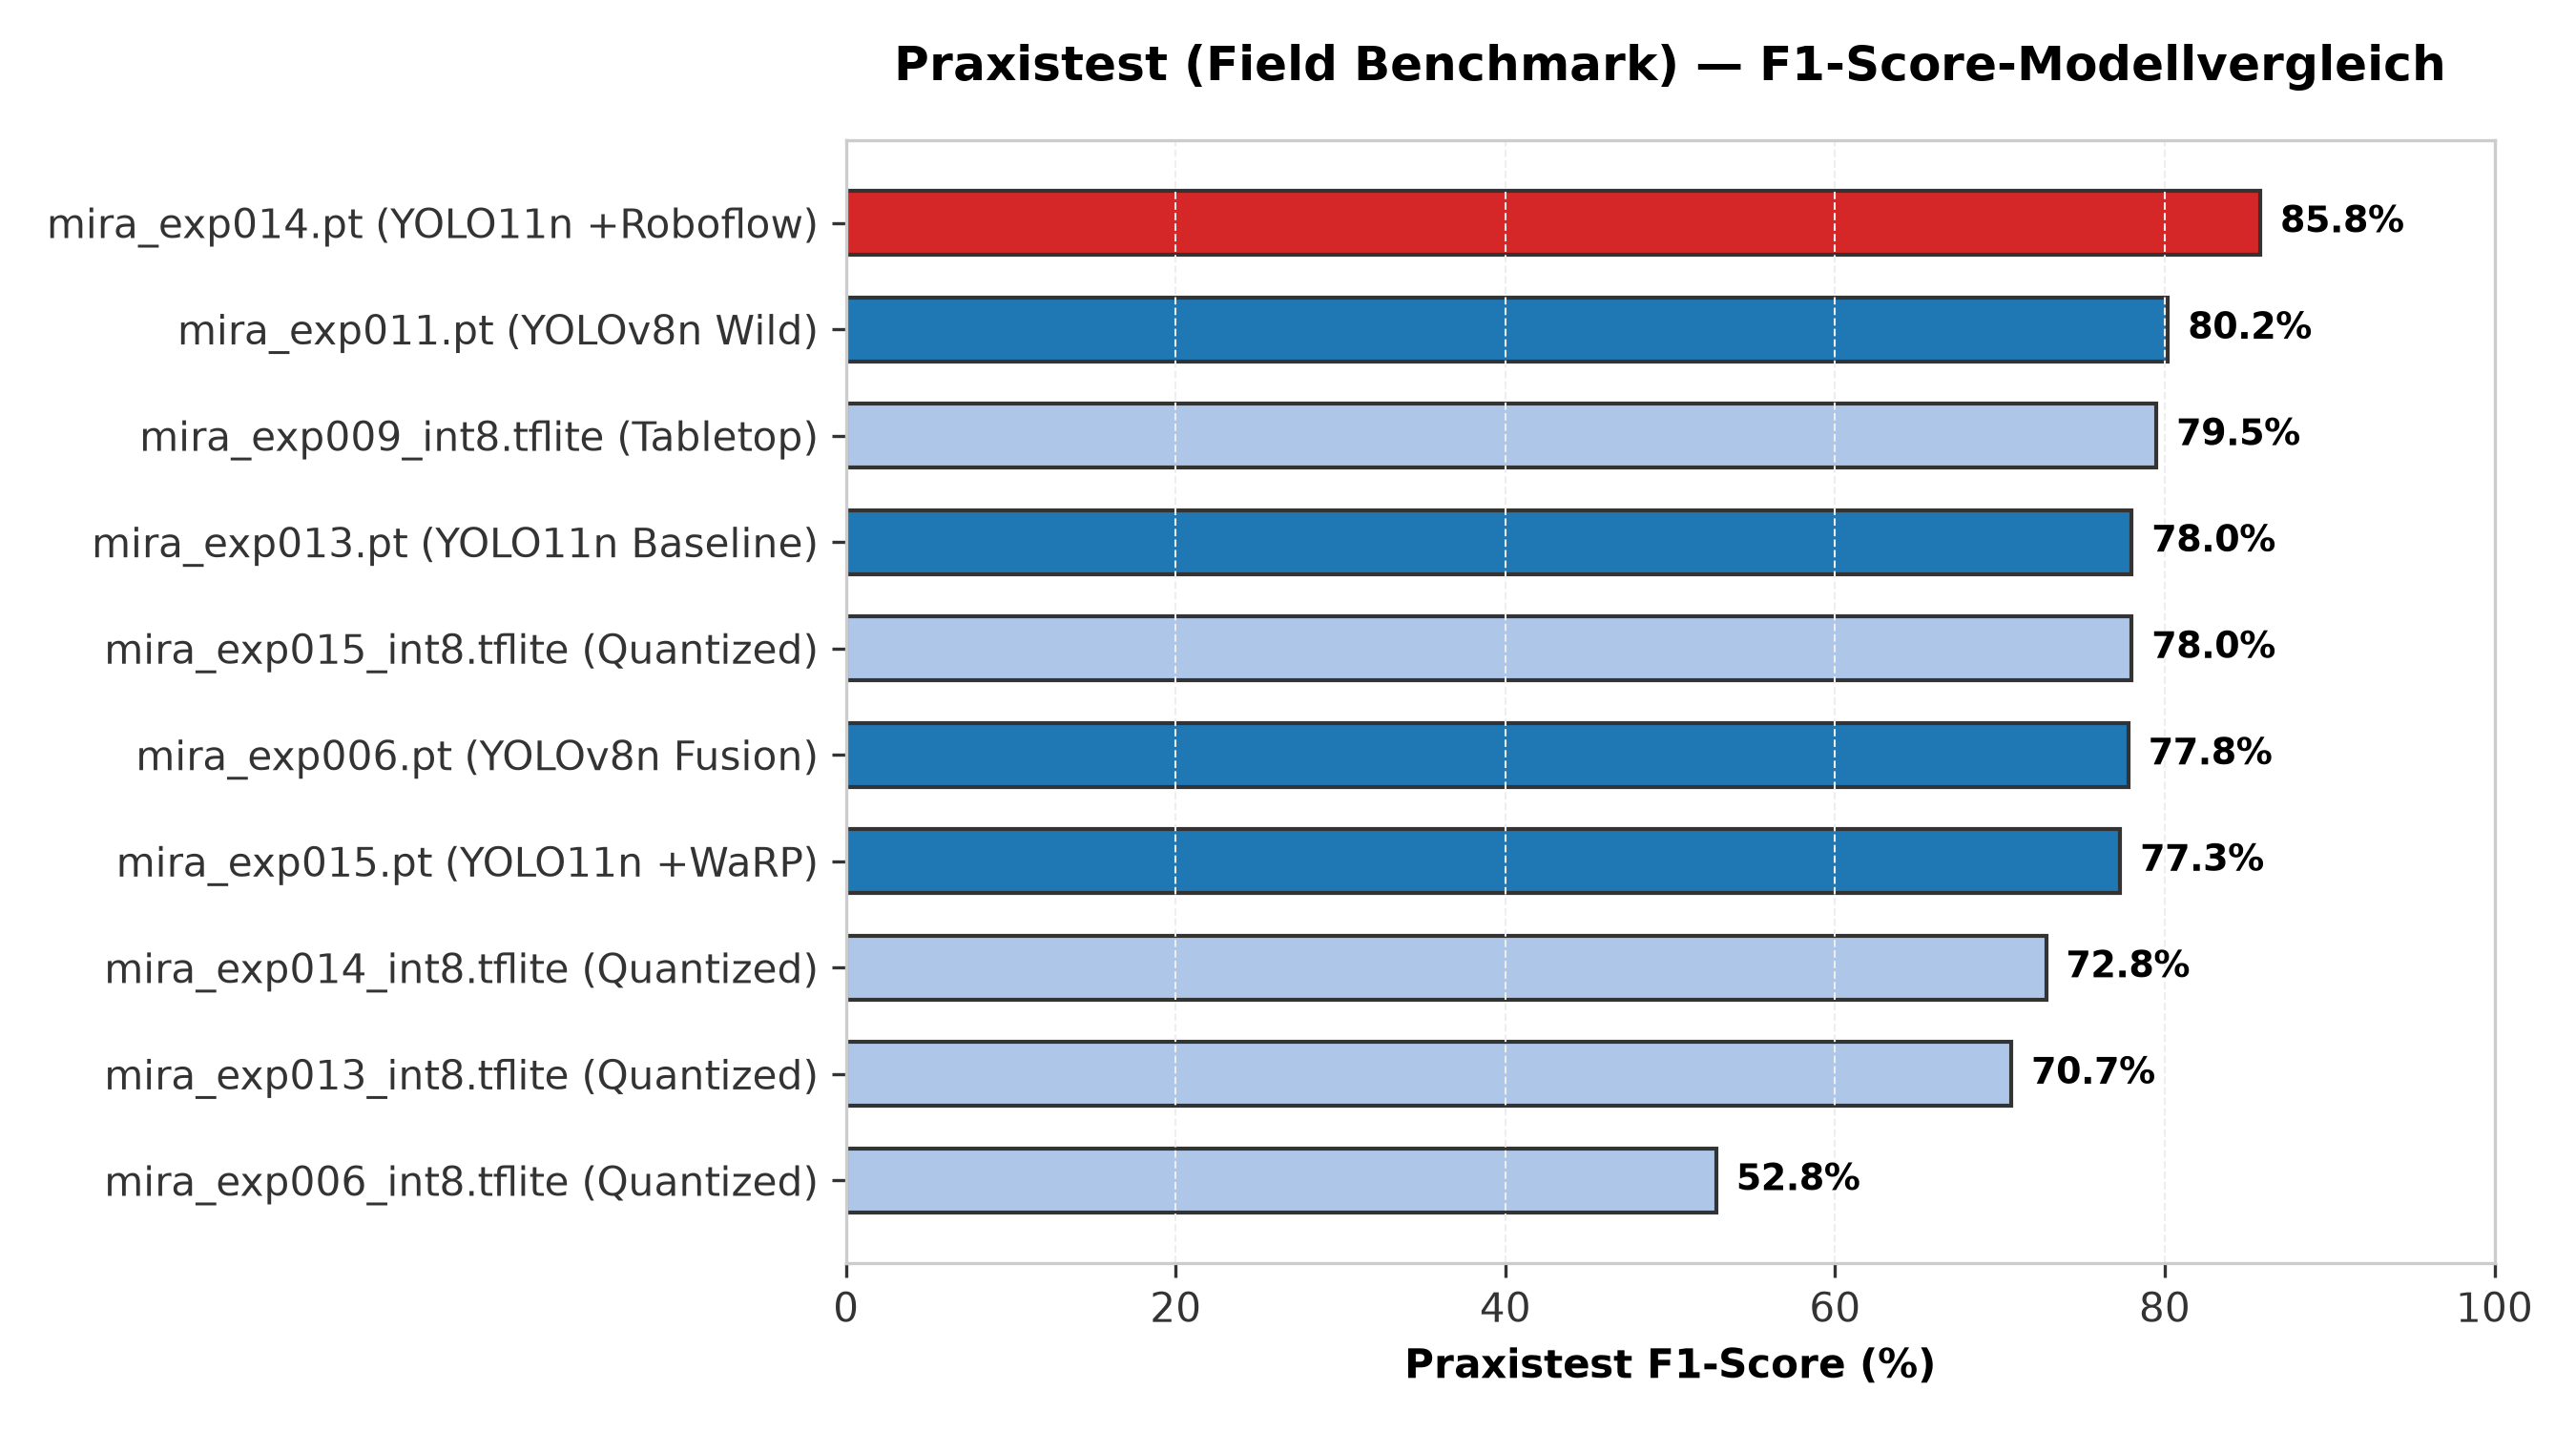
\includegraphics[width=0.95\textwidth, keepaspectratio]{figures/field-benchmark-f1.png}
    \caption{F1-Score-Vergleich aller getesteten Detektionsmodelle im Praxistest (Field Benchmark). Das Modell \texttt{mira\_exp014.pt} (EXP-014, YOLO11n auf TACO+TrashNet+Roboflow) erreicht mit \SI{85.8}{\percent} F1 den höchsten Wert. INT8-quantisierte Varianten zeigen durchweg einen F1-Verlust von ca. 13~pp.}
    \label{fig:field-benchmark-f1}
\end{figure}

Die klassenspezifischen F1-Scores des besten Modells (EXP-014) zeigt Tabelle~\ref{tab:exp014-field-class}.

\begin{table}[h]
    \centering
    \caption{Klassenspezifische F1-Scores von EXP-014 im Praxistest}
    \label{tab:exp014-field-class}
    \small
    \begin{tabular}{lccc}
        \toprule
        \textbf{Klasse} & \textbf{Precision} & \textbf{Recall} & \textbf{F1-Score} \\
        \midrule
        Glass   & \SI{93.0}{\percent} & \SI{86.9}{\percent} & \SI{89.9}{\percent} \\
        Metal   & \SI{89.2}{\percent} & \SI{81.1}{\percent} & \SI{84.9}{\percent} \\
        Paper   & \SI{94.6}{\percent} & \SI{87.2}{\percent} & \SI{90.7}{\percent} \\
        Plastic & \SI{96.8}{\percent} & \SI{82.3}{\percent} & \SI{88.9}{\percent} \\
        Trash   & \SI{75.5}{\percent} & \SI{42.0}{\percent} & \textbf{\SI{54.0}{\percent}} \\
\bottomrule
    \end{tabular}
\end{table}